% 04_csinet_quant.tex



While previous works investigated neural architectures for learned encoding-decoding of CSI data, such architectures rely on continuous valued latent representations (codewords). The use of such continuous codewords presents at least two issues:
\begin{enumerate}
	\item \textbf{Quantization}: Modulation protocols require quantized data to accommodate bit string representations and IQ constellations. To make neural autoencoders compatible with common modulation schemes, trainable CSI compression techniques should incorporate quantized codewords in the learning process.
	\item \textbf{Metrics for Compressibility}: Works in learnable CSI compression typically present a given network's reconstruction error a range of compression ratios (e.g., \cite{ref:csinet,ref:dualnet}) but do not discuss the network's compatibility with coding schemes. Coding techniques such as arithmetic coding \cite{ref:Witten1987Arithmetic}) require probability estimates of the encoded symbols in order to operate \cite{ref:Howard1994Arithmetic}. Based on Shannon's coding theorem \cite{ref:Shannon1948Mathematical}, the entropy of the encoded alphabet establishes is the minimum transmission rate needed to encode a given symbol. To describe their compatibility with optimal coding schemes, neural CSI compression techniques should be presented with the entropy of their encoded alphabets in order to assess the realized encoding distributions.
	% theory give metrics such entropy and mutual information which quantify the information in a given distribution.
\end{enumerate}

\subsection{Related Work}

Prior work has investigated feedback quantization in deep learning-based CSI compression. In \cite{ref:Yang2019DeepCMC}, the authors propose DeepCMC, an autoencoder structure where the continuous compressed elements are discretized via uniform quantization then encoded using context adaptive binary arithmetic coding (CABAC) \cite{ref:Marpe2003CABAC}. Since uniform quantization is non-differentiable, the authors do not perform true quantization during training and instead apply uniformly distributed noise to approximate quantization noise \cite{ref:Yang2019DeepCMC}. In \cite{ref:Mashhadi2020AnalogDeepCMC}, the authors propose AnalogDeepCMC, which encodes latent elements as power-normalized complex elements and decodes using maximal ratio combining. The authors also report the achieved rate of AnalogDeepCMC for different CSI overhead ratios.

To achieve discrete codewords with valid probability distributions, we consider works in neural discrete representations. In \cite{ref:Oord2017Neural}, the authors propose \emph{vector quantization (VQ)}, which partitions a $r$-dimensional latent space into $d$-dimensional vectors and quantizes the latent space based on a nearest neighbor assignment. In \cite{ref:Agustsson2017SoftToHard}, the authors proposed soft-to-hard VQ (SHVQ), a softmax relaxation of VQ which enables a latent entropy term which can be used to regularize the loss function.  Unlike the prior work, SHVQ allows for end-to-end training with feedback quantization.

\begin{figure}[!hbtp]
\centering
\def\svgwidth{0.8\columnwidth}
\input{../images/csinet_quant.pdf_tex}
\caption{Abstract architecture for CsiNet-Quant. SoftQuantize layer ($Q(\tilde{\mathbf Z})$) is a continuous, softmax-based relaxation of a $d$-dimensional quantization of the latent layer $\mathbf Z$.}
\label{fig:csinet_quant}
\end{figure}

\subsection{A Vector Quantized Autoencoder for Trainable Codewords}
% \subsubsection{CsiNet-Quant: A Vector Quantized Autoencoder for Trainable Codewords}

To incorporate discrete latent codewords in the learning process, we propose to use soft-to-hard vector quantization framework proposed in \cite{ref:Agustsson2017SoftToHard}. We choose a vector dimension, $m$, by which to partition the latent space $\mathbf Z = f(\mathbf H, \theta_e)$, and we denote the vectorized version of $\mathbf Z \in \mathbb R^{r}$ as $\tilde{\mathbf Z} \in \mathbb R^{r/m \times m}$. We define the $m$-dimensional codebook of size $L$ as $\mathbf C \in \mathbb R^{m\times L}$. The soft assignments of the $j$-th latent vector $\tilde{\mathbf z}_j$ can be written as
\begin{align}
\phi(\tilde{\mathbf z}_j) &= \left[\frac{\text{exp}(-\sigma \Arrowvert \tilde{\mathbf z}_j - \mathbf c_\ell\Arrowvert^2)}{\sum_{i=1}^L\text{exp}(-\sigma \Arrowvert \tilde{\mathbf z}_j - \mathbf c_i\Arrowvert^2)}\right]_{\ell\in [L]} \in \mathbb R^L \label{eq:soft_assign}
\end{align}
(\ref{eq:soft_assign}) is typically referred to as the \emph{softmax} function, which is commonly used as a differentiable alternative to the maximum function in deep learning. The hyperparameter $\sigma$ controls the temperature of the softmax scores, with a lower $\sigma$ yielding a more uniform distribution and a higher $\sigma$ yielding a ``peakier'' distribution (i.e., $\sigma \to \infty \Rightarrow \phi(\tilde z_j) \to \text{max}(\tilde z_j)$). Using the soft assignments, the latent vectors are quantized based on the codewords $\mathbf C \in \mathbb R^{m \times L}$,
\begin{align}
Q(\tilde{\mathbf z}_j,\mathbf C) &= \phi(\tilde{\mathbf z}_j) \mathbf C^T. \label{eq:soft_quant}
\end{align}
The quantized version of the latent variable is taken by reshaping $\mathbf Q(\tilde{\mathbf Z},\mathbf C) \in \mathbb R^{r/m \times m}$ into $\hat{\mathbf Z} \in \mathbb R^d$, and the decoder produces the CSI estimates as $\hat{\mathbf H} = h(\hat{\mathbf Z}, \mathbf C)$. An abstract illustration of an autoencoder using soft quantization can be seen in Figure~\ref{fig:csinet_quant}.

\subsubsection{Entropy-regularization}
To optimize the network with soft quantization, we adapt the loss function to resemble the canonical rate-distortion function by adding an entropy penalization term,
\begin{align}
\underset{\theta_e, \theta_d, \mathbf C}{\text{argmin}}\; \frac 1N \underbrace{\sum_{i=1}^N\Arrowvert \mathbf H_i - g(Q(f(\mathbf H_i, \theta_e), \mathbf C), \theta_d) \Arrowvert^2}_{\text{distortion loss}} + \underbrace{\lambda \left(\Arrowvert\theta_e\Arrowvert^2+\Arrowvert\theta_d\Arrowvert^2+\Arrowvert \mathbf C \Arrowvert^2\right)}_{\ell^2\text{ penalty}} + \underbrace{m\beta H(\phi)}_{\text{rate loss}}. \label{eq:loss_entropy}
\end{align}
Where $H(\phi)=H(p,q)$ is the crossentropy based on the hard and soft probability estimates $p$ and $q$, respectively. Before defining the estimates $p$ and $q$, we briefly discuss the population probabilities of the latent codewords. Denote the symbol encoder/decoder pair as $E:\mathbb R^m \to [L]^m$/$D:[L]^m \to \mathbb R^m$. Denote the distribution of latent variables as $\mathsf Z$ such that $\mathbf z \sim \mathsf Z$ with the encoder $E(\mathsf Z)=\mathbf e$ . The entropy of $\mathsf Z$ is given as 
\begin{align*}
H(E(\mathsf Z)) &= -\sum_{\mathbf e\in[L]^m}P(E(\mathsf Z) = \mathbf e)\log_2(P(E(\mathsf Z)=\mathbf e)).
\end{align*}
% The true probabilities over the latent vectors as $p_j$ with entropy $H(p) = -\sum_{j}^m p_j\log_2 p_j$.
In practice, the true population probabilities $P(E(\mathsf Z))$ are inaccessible, and we must estimate the probability masses via finite sampling over the encoder's outputs, $e(\mathbf z)$. The hard probability estimate $p_j$ of the $j$-th codeword is
\begin{align*}
p_j &= \frac{|\{e_l(\mathbf z_i)|l\in[m], i \in [N], e_l(\mathbf z_i)=j\}|}{mN}.
\end{align*}
The soft assignments of $\phi$ admit valid probability masses, $q_j = \phi(\tilde{\mathbf z})$, over the codewords. Using histogram estimates $p_j$ and the soft assignments $q_j$, the crossentropy term is written
\begin{align*}
H(\phi) := H(p,q) &= -\sum_{j=1}^L p_j\log q_j = H(p) + D_{\text{KL}}(p\Arrowvert q)
\end{align*}
where $D_{\text{KL}}(p\Arrowvert q)=-\sum_{j=1}^L p_j \log\left(\frac{p_j}{q_j}\right)$ is the Kullback Liebler (KL) divergence. Due to the nonnegativity of $D_{\text{KL}}$, $H(\phi)$ is an upper bound on $H(p)$, and so (\ref{eq:loss_entropy}) is a valid optimization target.

The mean squared error of the soft (hard) network is given as $e_S=\Arrowvert \tilde F(\mathbf H) - \mathbf H\Arrowvert^2$ ($e_H=\Arrowvert \hat F(\mathbf H) - \mathbf H\Arrowvert^2$), and the performance gap is given as $\text{gap}(t)=e_H - e_S$.

\subsection{Results}

We use SHVQ \cite{ref:Agustsson2017SoftToHard} to perform quantization on different CSI estimation networks. We used the COST2100 data introduced in Section~\ref{sect:channel_model}. We train the network in three stages:
\begin{enumerate}
	\item \textbf{Autoencoder pretraining}: Training the autoencoder ($\hat{\mathbf{H}}=g(f(\mathbf H, \vec\theta_e), \vec\theta_d)$) without latent quantization (1000 epochs). The autoencoder is trained with the MSE objective function.
	\item \textbf{Center pretraining}: Training soft quantization layer to initialize centers, $\mathbf C$ (1000 epochs). Using $\vec \theta_e$ from stage 1, the soft quantizer is trained on $\mathbf Z=f(\mathbf H, \vec \theta_e)$ to minimize the cluster energy, $\underset{\mathbf C}{\text{argmin}}\sum_{i=1}^N \Arrowvert \tilde{\mathbf Z} - Q(\tilde{\mathbf Z})\Arrowvert^2$.
	\item \textbf{SHVQ finetuning}: Using the results of stage 1 ($\vec\theta_e, \vec\theta_d$) and stage 2 ($\mathbf C$), we finetune the autoencoder and the soft quantization layer (50 epochs). The soft-quantized autoencoder is trained with the entropy-regularized MSE (Equation (\ref{eq:loss_entropy})).
\end{enumerate}

We use a batch size of 200. We perform a training/testing split of 75k/25k sample. For stage 3, we sweep the parameter $\beta$ to realize different latent entropy values $H(\phi)$. To visualize the rate-distortion of the proposed network, we show the network's NMSE versus the bits per pixel (bpps), 
\begin{align*}
	\text{bpps}	 &= \frac{rm}{2 n_{b}R_{d}}H(\phi) = CR\times mH(\phi). % bpps = test_entropy * (model.latent_dim / model.quant.m) / (2*model.decoder.img_total) # bits per pixel
\end{align*}
We also perform experiments with arithmetic encoding on the hard quantized centers, and we report the resulting bits per pixel as
\begin{align*}
	\text{bpps}	 &= \frac{\frac 1N \sum_{i}^N b_{\text{AE}}}{2 n_{b}R_{d}}. % bpps = test_entropy * (model.latent_dim / model.quant.m) / (2*model.decoder.img_total) # bits per pixel
\end{align*}
where $b_{\text{AE}}$ is the average bits per feedback message under arithmetic encoding.

We demonstrate the performance of CsiNet, SphNet, and DualNet-MAG under latent quantization. Table~\ref{tab:quant-params} summarizes the parameters used in these tests.

\begin{table}[]
\centering
\caption{Parameters/hyperparameters used for CsiNet-Quant.}
\label{tab:quant-params}
\begin{tabular}{c|c|l}
\toprule
\textbf{Symbol}   & \textbf{Values}  & \textbf{Description} \\ \midrule
$L$ 		  	  & $1024$	 		 & Number of centers/codewords for VQ.  \\ \hline
$d$               & $4$				 & Dimensionality of vectors in VQ.  \\ \hline
$r$               & $4$				 & Number of elements at the encoder's output (i.e., dimension of latent layer).  \\ \hline
\end{tabular}
\end{table}

\subsubsection{Rate-Distortion}

Figures~\ref{fig:rate-distortion-minmax} and~\ref{fig:rate-distortion-sph} show the performance of CsiNet-Quant under minmax and spherical normalization, respectively. 

\begin{figure}[htb] \centering 
  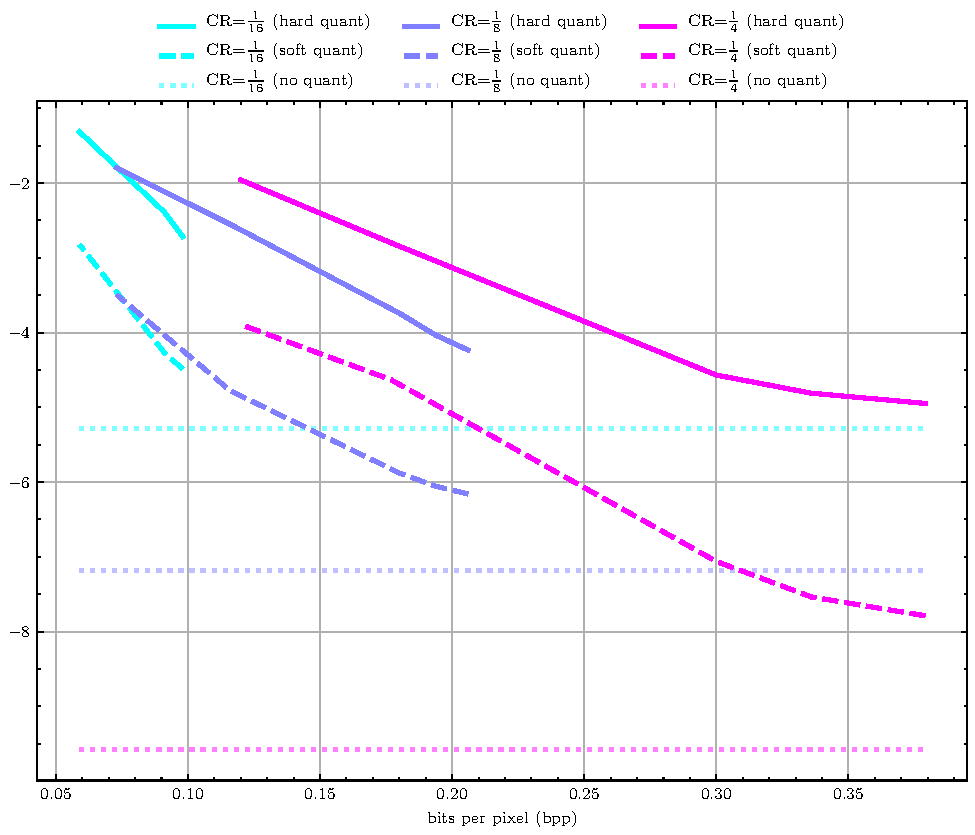
\includegraphics[width=0.8\linewidth]{rate-distortion-all-cr-H4.pdf}
  \caption{Rate distortion of CsiNet-Quant under minmax normalization using: $L=1024$ centers, $d=4$. Hard, soft, and no quantization performance shown for each CR.} 
  \label{fig:rate-distortion-minmax} 
\end{figure}

\begin{figure}[htb] \centering 
  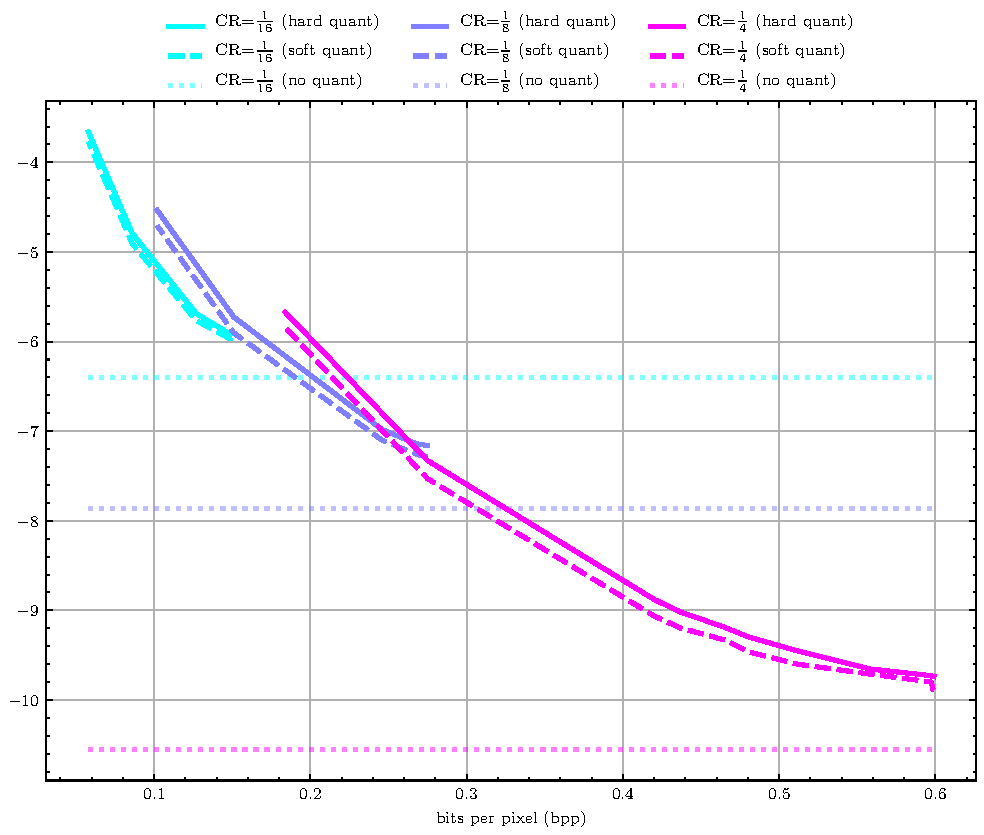
\includegraphics[width=0.8\linewidth]{rate-distortion-all-cr-sphH4.pdf}
  \caption{Rate distortion of CsiNet-Quant under spherical normalization using: $L=1024$ centers, $d=4$. Hard, soft, and no quantization performance shown for each CR.} 
  \label{fig:rate-distortion-sph} 
\end{figure}

\begin{figure}[htb] \centering 
  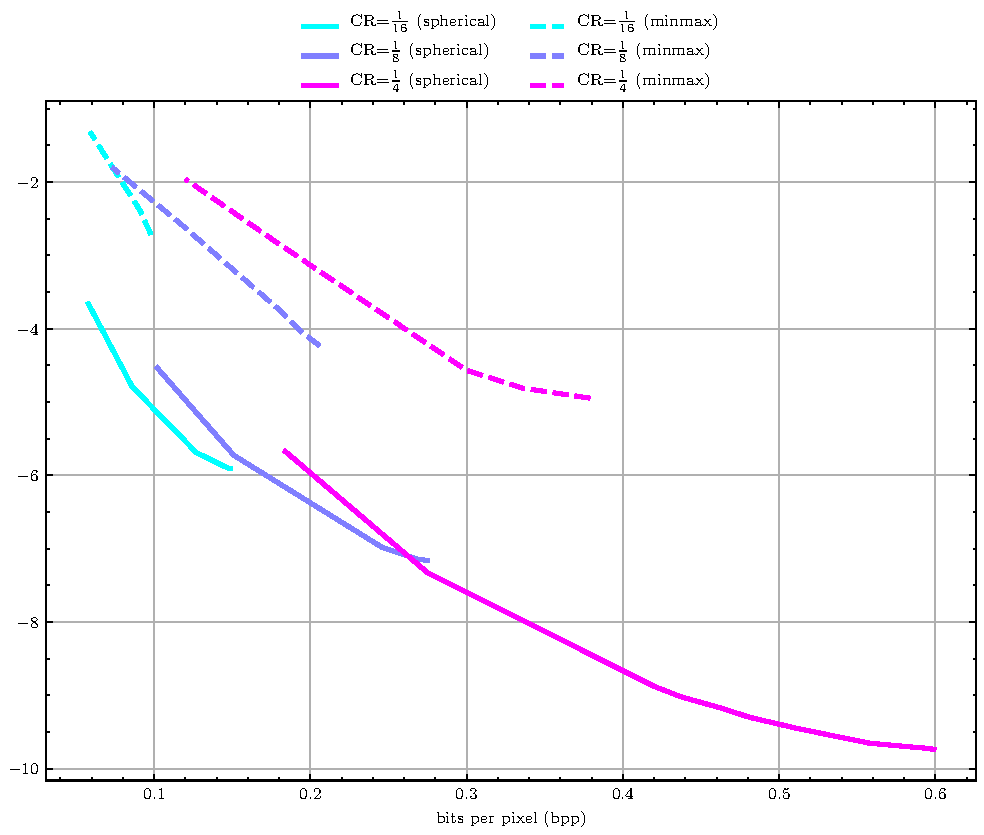
\includegraphics[width=0.8\linewidth]{rate-distortion-all-norm.pdf}
  \caption{Rate distortion under hard quantization for both minmax (dotted line) and spherical (solid line) normalization using.} 
  \label{fig:rate-distortion-norms} 
\end{figure}

% Open Questions:
% Metrics for Compressibility:
% - Rate calculation: Can depend on
% 	- Precoding technique (conjugate beamforming, zero-forcing)
% 	- SNR in Uplink/Downlink
% - Entropy:
%	- Latent entropy estimation enables rate-loss
% 	- Raw entropy estimation techniques?
%		- Discrete: Questions of quantization resolution
%		- Continuous: Questions of hyperparameters for density-estimatiors (i.e., KNN)
% - Realized Bitrate under Entropy Encoding
% 	- Given rate-regularized training, what is the average Tx bit rate under an entropy encoding scheme?
% 		- Start with Arithmetic Codin
%		- Move onto Context-adaptive binary arithmetic coding